% указываем класс документа
\documentclass[12pt,a4paper,openany]{extarticle}

% подключаем собственный стилевой файл 
\usepackage{mystyle}

% указываем язык (для автоматической вставки слов, типа "Глава", "Содержание", "Литература", "рис." и пр.
\selectlanguage{russian}

\begin{document}
\part*{Маятник Фуруты}

\begin{figure}[h]
	\noindent\centering{ 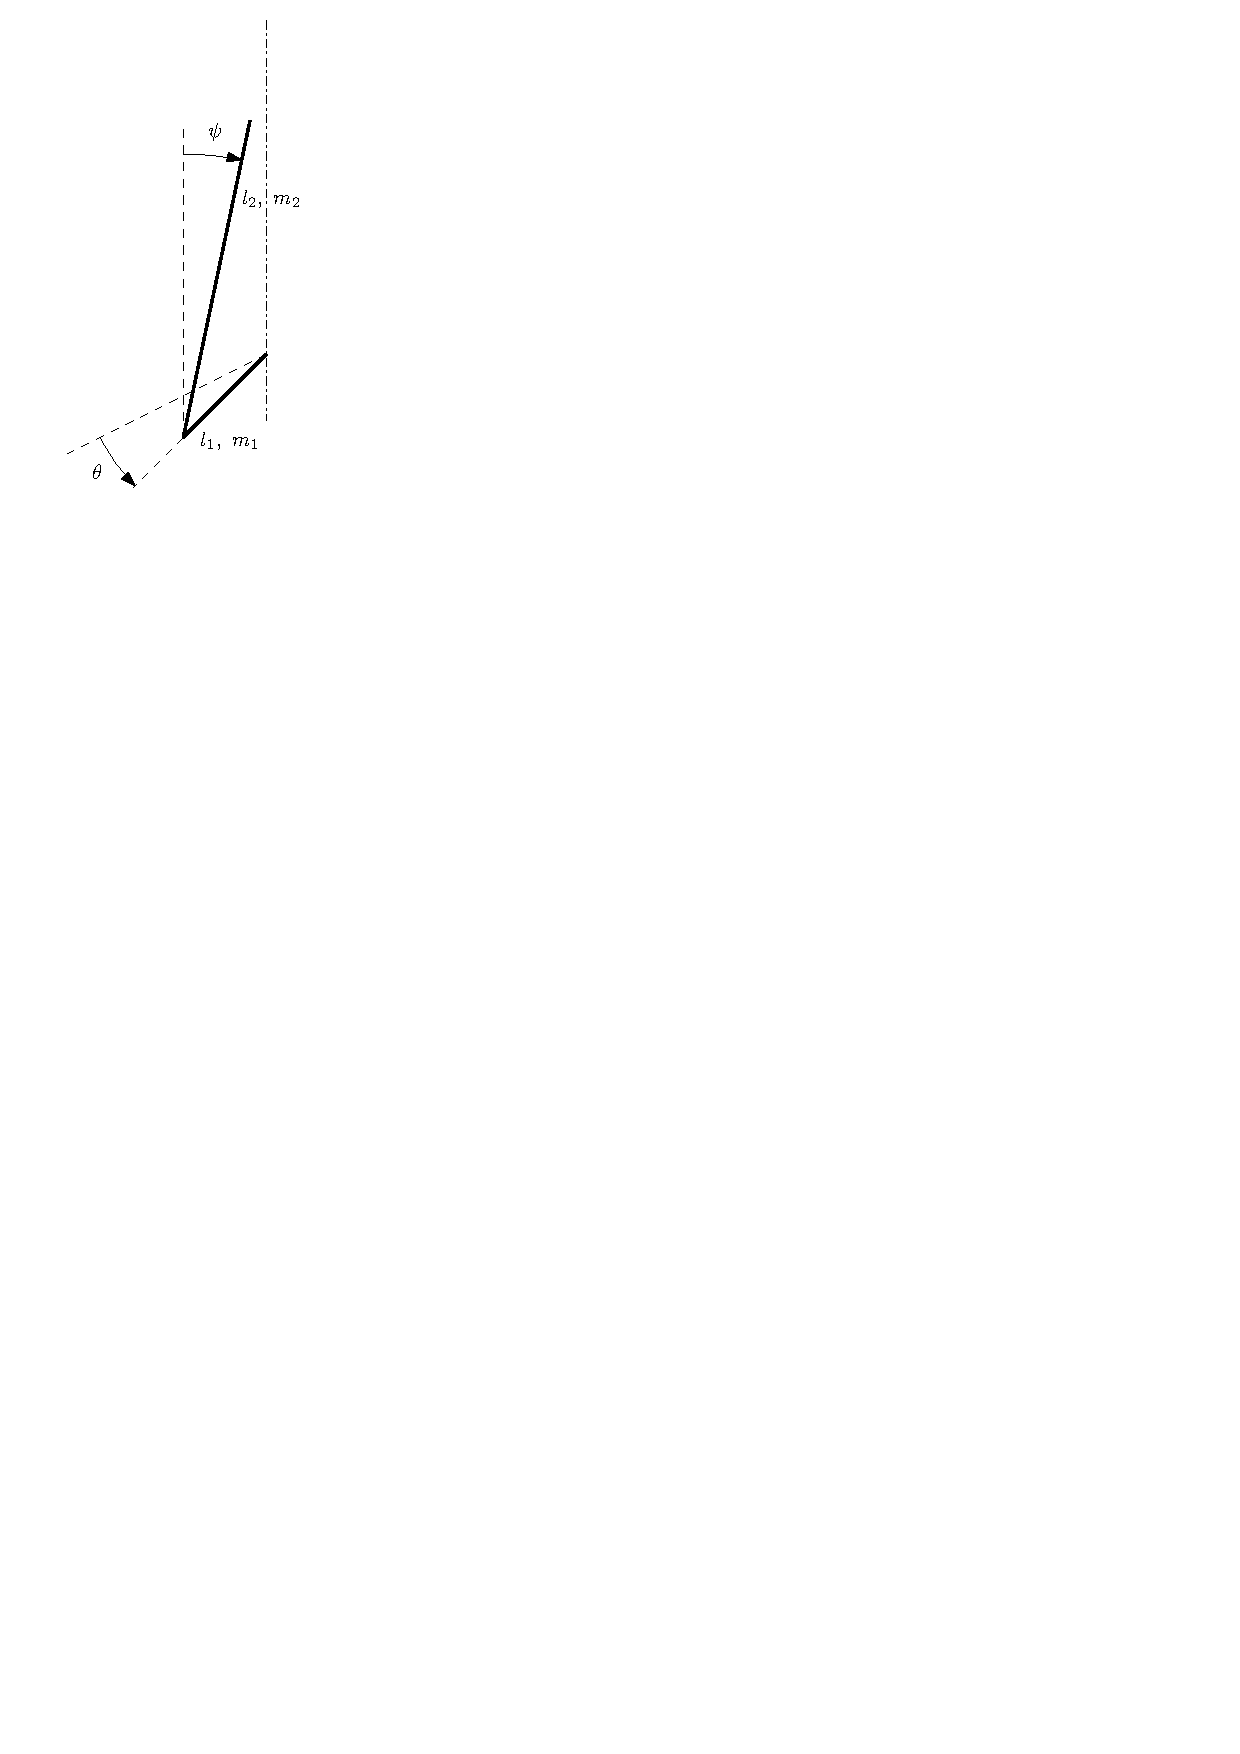
\includegraphics[scale=1.5]{furuta.pdf} }
	\caption{Схема робота.}
	\label{fig:scheme_of_robot}
\end{figure}

\begin{equation}
E = 
\begin{bmatrix}
4m_2l_1^2+m_1l_1^2+4I_{z2}+4I_{y1}+4J & 2m_2l_1l_2 \\
2m_2l_1l_2 & 4I_{y2}+m_2l_2^2
\end{bmatrix}
\quad
F = 
\begin{bmatrix}
\cfrac{4k_mk_e}{R} & 0\\
0 & 0
\end{bmatrix}
\end{equation}

\begin{equation}
G = 
\begin{bmatrix}
0 & 0\\
0 & -2m_2gl_2
\end{bmatrix}
\quad
H = 
\begin{bmatrix}
\cfrac{4k_m}{R}\\
0
\end{bmatrix}
\end{equation}

\begin{equation}
Q_1 = -E^{-1}F \qquad Q_2 = -E^{-1}G \qquad Q_3 = E^{-1}H
\end{equation}


\begin{equation}
A = 
\begin{bmatrix}
0 & 0 & 1\\
Q_2(1,2) & Q_1(1,1) & 0\\
Q_2(2,2) & Q_1(2,1) & 0
\end{bmatrix}
\qquad
B= 
\begin{bmatrix}
0 \\ Q_3(1,1) \\ Q_3(2,1)
\end{bmatrix}
\end{equation}

\end{document}